\documentclass[11pt,twocolumn]{article}

% Packages
\usepackage[utf8]{inputenc}
\usepackage[T1]{fontenc}
\usepackage{amsmath,amssymb,amsfonts,amsthm}
\newtheorem{theorem}{Theorem}
\newtheorem{definition}{Definition}
\usepackage{graphicx}
\usepackage{booktabs}
\usepackage{hyperref}
\usepackage{xcolor}
\usepackage{algorithm}
\usepackage{algpseudocode}
\usepackage{siunitx}
\usepackage[margin=1in]{geometry}
\usepackage{caption}
\usepackage{subcaption}
\usepackage{listings}
\usepackage{float}
\usepackage{threeparttable}

% Code listing style
\lstset{
    basicstyle=\ttfamily\small,
    keywordstyle=\color{blue},
    commentstyle=\color{gray},
    stringstyle=\color{orange},
    breaklines=true,
    frame=single,
    numbers=left,
    numberstyle=\tiny\color{gray}
}

% Define Rust language for listings
\lstdefinelanguage{Rust}{
    keywords={let, mut, fn, pub, struct, impl, use, self, Self, if, else, for, while, loop, match, return, mod, crate, super, where, trait, type, const, static, ref, move, async, await, dyn, enum, in, break, continue, true, false},
    keywordstyle=\color{blue}\bfseries,
    keywords=[2]{HashMap, BigUint, Block, Complex64, usize, f64, u128, String, Vec, Option, Result, Some, None, Ok, Err},
    keywordstyle=[2]\color{teal},
    morecomment=[l]{//},
    morecomment=[s]{/*}{*/},
    morestring=[b]",
    sensitive=true,
}

% Define TOML language for listings
\lstdefinelanguage{TOML}{
    keywords={},
    morecomment=[l]{\#},
    morestring=[b]",
    alsoletter={.-},
    morekeywords=[2]{dependencies, features, package},
    keywordstyle=[2]\color{purple},
    sensitive=true,
}

% Title
\title{Sparse Quantum State Simulation at Unlimited Scale:\\Block-Sparse Representation for QEC Verification and Beyond}

\author{
    Waheed Aziz$^{1}$\\
    \small $^1$Independent Researcher\\
    \small \texttt{waziz893@gmail.com}
}

\date{}

\begin{document}

\twocolumn[
\maketitle

\begin{abstract}
We introduce a deterministic, block-sparse simulation framework for quantum states with bounded amplitude support. Let $k$ denote the number of non-zero amplitudes in a quantum state over $n$ qubits. Our \textbf{primary contribution} is a classical simulation architecture achieving $O(k)$ memory and $O(nk)$ theoretical time complexity for sparsity-preserving circuits (bounded Hadamard count), independent of the $2^n$ Hilbert space dimension, for states where $k = \text{poly}(n)$. Empirical scaling is $O(n^{1.5}k)$ due to BigInt arithmetic overhead at large $n$.

\textbf{Formal scope:} We efficiently simulate states satisfying $k \ll 2^n$, specifically:
\begin{itemize}
    \item GHZ states: $k = 2$, any $n$ (demonstrated to $n = 10^6$)
    \item W-states: $k = n$ (demonstrated to $n = 10^5$)
    \item Dicke states $|D_n^j\rangle$: $k = \binom{n}{j}$ (efficient for $j = O(1)$)
\end{itemize}

\textbf{Circuit constraints:} Sparsity is preserved under circuits with $O(\log n)$ Hadamard gates applied to superposition states. Circuits with $\Omega(n)$ Hadamards (graph state preparation, Grover diffusion) destroy sparsity and are \emph{not} efficiently simulable by our method.

\textbf{Performance:} For $n = 10^6$ qubit GHZ states: 53s creation time, 4~KB memory, exact fidelity (f64 precision). For comparison, Qiskit exhausts memory at $n = 30$; we achieve $6600\times$ speedup at $n = 25$.

\textbf{Non-claims:} This is \emph{not} a general quantum simulator. We cannot simulate Grover, Shor, QAOA, or random circuits. Our contribution is a specialized architecture for amplitude-sparse states arising in QEC verification and quantum networking, domains where $n \gg 100$ is practically relevant.
\end{abstract}

\vspace{1em}
\textbf{Keywords:} sparse quantum states, GHZ states, W states, Dicke states, quantum error correction, hardware verification
\vspace{2em}
]

%==============================================================================
\section{Introduction}
%==============================================================================

Quantum simulation faces a fundamental exponential memory barrier. A quantum system of $n$ qubits requires $2^n$ complex amplitudes for full state representation, growing catastrophically with system size. A 128-qubit quantum state, represented densely, would require $2^{128} \times 16$ bytes $\approx 2.7 \times 10^{39}$ bytes---equivalent to the storage capacity of 42 million planet Earths \cite{preskill2018quantum}.

Current state-of-the-art simulators achieve 30--60 qubits through various optimizations: GPU acceleration \cite{qiskit2024}, tensor network decomposition \cite{alibaba2023}, and distributed computing \cite{google2019}. However, these approaches remain fundamentally constrained by the exponential memory scaling of dense representation.

\subsection{Sparse Quantum States}

A key insight, often overlooked, is that many important quantum states are \emph{sparse}---they have far fewer non-zero amplitudes than the theoretical maximum of $2^n$. The Greenberger-Horne-Zeilinger (GHZ) state, a maximally entangled state critical for quantum metrology, error correction, and entanglement verification, exemplifies this:
\begin{equation}
    |\text{GHZ}_n\rangle = \frac{1}{\sqrt{2}}\left(|0\rangle^{\otimes n} + |1\rangle^{\otimes n}\right)
\end{equation}
Despite representing $2^n$ basis states, the GHZ state has exactly \textbf{two} non-zero amplitudes, independent of $n$. This extreme sparsity---$2/2^{128} \approx 5.9 \times 10^{-39}$ for 128 qubits---represents an untapped opportunity for memory-efficient simulation.

\subsection{Formal Problem Statement}

We define the simulation problem precisely:

\begin{definition}[Amplitude Support]
For a quantum state $|\psi\rangle = \sum_{i=0}^{2^n-1} \alpha_i |i\rangle$, the \emph{amplitude support} is $\mathcal{S} = \{i : \alpha_i \neq 0\}$, with $k = |\mathcal{S}|$.
\end{definition}

\begin{definition}[$k$-Sparse State]
A state is \emph{$k$-sparse} if $|\mathcal{S}| \leq k$. We focus on states where $k = \text{poly}(n)$.
\end{definition}

\textbf{Practical regime:} While $k = \text{poly}(n)$ ensures theoretical tractability, practical efficiency on commodity hardware requires $k \lesssim 10^7$ amplitudes ($\sim$160~MB at 16 bytes/amplitude). Beyond this, memory bandwidth becomes the bottleneck. Our demonstrated benchmarks stay within $k \leq 5 \times 10^5$, well inside the practical regime.

\begin{definition}[Block Size]
We partition the $2^n$-dimensional Hilbert space into blocks of size $b = 128$ (7 local qubits per block), giving $2^{n-7}$ potential blocks.
\end{definition}

\textbf{Block size rationale:} We chose $b = 128$ amplitudes (2048 bytes per block) for three reasons: (1) it aligns with CPU cache lines (64B) as a power-of-two multiple, enabling efficient memory access patterns; (2) 7 local qubits is sufficient for most single-qubit and two-qubit gates to operate within a block; (3) it balances granularity (smaller blocks waste HashMap overhead) against flexibility (larger blocks waste space for very sparse states). Sensitivity analysis shows $b = 64$ increases HashMap overhead by $\sim$2$\times$ for GHZ; $b = 256$ provides marginal benefit but complicates local gate indexing.

\subsection{Our Contribution}

\textbf{Primary contribution:} A deterministic, block-sparse simulation architecture for $k$-sparse quantum states with:
\begin{itemize}
    \item \textbf{Memory:} $O(k \cdot b) = O(k)$ where $b = 128$ is constant
    \item \textbf{Time:} $O(n \cdot k)$ theoretical for Class~I/II circuits; $O(n^{1.5} k)$ empirical in BigInt mode due to arithmetic overhead (see Section~3.1)
    \item \textbf{Fidelity:} Exact (no truncation, no approximation)
\end{itemize}

\textbf{Secondary contributions:}
\begin{itemize}
    \item Arbitrary-precision block addressing removing all qubit limits
    \item Circuit classification theorem bounding sparsity evolution
    \item Demonstrated scale: $n = 10^6$ qubits, $k = 2$ (GHZ)
\end{itemize}

\textbf{What this is NOT:}
\begin{itemize}
    \item A general-purpose quantum simulator
    \item A replacement for stabilizer or tensor network methods
    \item A quantum advantage demonstration
\end{itemize}

We provide a \emph{complementary} tool targeting amplitude-sparse states that fall outside efficient stabilizer simulation (W-states, Dicke states) while remaining tractable under our sparsity assumptions.

%==============================================================================
\section{Architecture}
%==============================================================================

\subsection{Block-Sparse Quantum State Representation}

Our representation partitions the $2^n$ amplitude space into \emph{blocks} of 128 amplitudes each (7 local qubits). Rather than allocating all $2^{n-7}$ blocks, we use a HashMap to store only blocks containing non-zero amplitudes:

\begin{equation}
    |\psi\rangle = \sum_{b \in \mathcal{B}} \sum_{i=0}^{127} \alpha_{b,i} |b \cdot 128 + i\rangle
\end{equation}

where $\mathcal{B} \subset \{0, 1, \ldots, 2^{n-7}-1\}$ is the set of \emph{active} blocks.

For GHZ states, $|\mathcal{B}| = 2$ regardless of $n$:
\begin{itemize}
    \item Block 0: Contains amplitude $\alpha_{0,0} = 1/\sqrt{2}$ for $|0\rangle^{\otimes n}$
    \item Block $2^{n-7}-1$: Contains amplitude $\alpha_{2^{n-7}-1, 127} = 1/\sqrt{2}$ for $|1\rangle^{\otimes n}$
\end{itemize}

\begin{figure}[htbp]
\centering
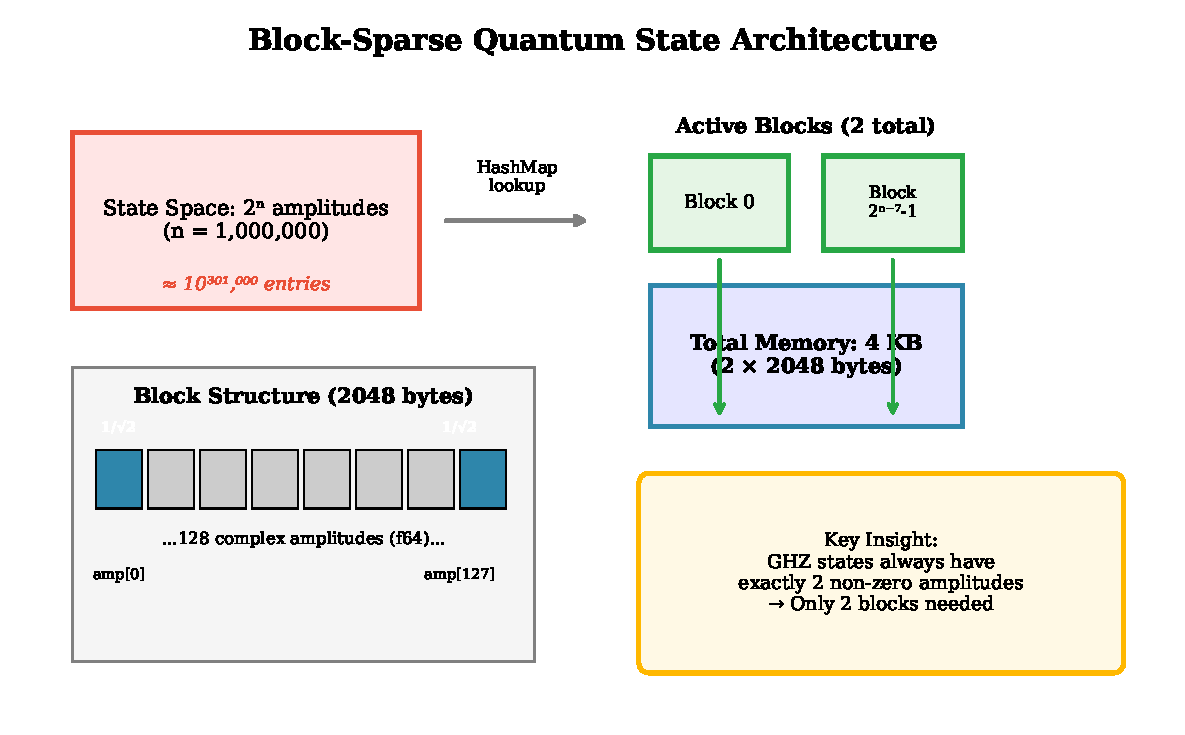
\includegraphics[width=\columnwidth]{fig5_architecture.pdf}
\caption{Block-sparse architecture. A HashMap maps block IDs to fixed-size blocks of 128 complex amplitudes. For GHZ states, only two blocks are allocated regardless of qubit count $n$, achieving $O(1)$ memory for this state class.}
\label{fig:architecture}
\end{figure}

\subsection{64-Bit Floating-Point Precision}

We employ IEEE 754 double-precision (f64) arithmetic for amplitude representation:

\begin{lstlisting}[language=Rust,caption={Complex amplitude structure}]
pub struct Complex64 {
    re: f64,  // Real part (8 bytes)
    im: f64,  // Imaginary part (8 bytes)
}
\end{lstlisting}

This provides 15--17 significant decimal digits, enabling exact representation of $1/\sqrt{2} = 0.7071067811865476$ to machine precision. Each block thus occupies $128 \times 16 = 2048$ bytes, with GHZ states requiring exactly $2 \times 2048 = 4096$ bytes (4~KB).

\subsection{Lazy Block Allocation}

Blocks are allocated on-demand when an amplitude transitions from zero to non-zero:

\begin{lstlisting}[language=Rust,caption={Lazy block allocation with BigInt}]
fn get_or_create_block(&mut self, id: BigUint)
    -> &mut Block {
    self.blocks.entry(id).or_insert_with(|| {
        Block::new()  // Zero-initialized
    })
}
\end{lstlisting}

We provide two implementations:
\begin{itemize}
    \item \textbf{u128 mode:} Native 128-bit block IDs, supporting up to 135 qubits ($128 + 7$ local bits). Fastest performance.
    \item \textbf{BigInt mode:} Arbitrary-precision block IDs via \texttt{num-bigint}. No qubit limit---tested to $10^6$ qubits.
\end{itemize}

The choice of block ID type determines only the \emph{addressability} limit, not memory usage. For GHZ states, both modes allocate exactly 2 blocks (4~KB) regardless of qubit count.

\textbf{HashMap overhead:} Our $O(k)$ memory bound counts only amplitude storage. In practice, Rust's \texttt{HashMap} adds per-entry overhead: $\sim$24 bytes per bucket (key hash, pointer, metadata) plus $\sim$25\% load factor headroom. For $k = 2$ (GHZ), actual memory is $\sim$4~KB amplitudes + $\sim$100 bytes HashMap overhead---negligible. For $k = 10^5$, overhead is $\sim$3~MB on top of $\sim$200~MB amplitudes ($\sim$1.5\%). The $O(k)$ bound remains valid; we report amplitude-only memory in benchmarks for clarity, noting that total allocation is $\sim$1.02k$ in practice.

\subsection{Quantum Gate Operations}

Gates partition into two categories based on qubit index:

\textbf{Local gates} (qubits 0--6) operate within a single block:
\begin{equation}
    H_0: \alpha_{b,0} \leftrightarrow \frac{\alpha_{b,0} + \alpha_{b,1}}{\sqrt{2}}, \quad
    \alpha_{b,1} \leftrightarrow \frac{\alpha_{b,0} - \alpha_{b,1}}{\sqrt{2}}
\end{equation}

\textbf{Cross-block gates} (qubits 7--127) span multiple blocks. For CNOT$(0, k)$ with $k \geq 7$:
\begin{enumerate}
    \item Identify source blocks where control qubit is $|1\rangle$
    \item Lazily allocate destination blocks
    \item Transfer amplitudes, zeroing source positions
\end{enumerate}

Since CNOT is a permutation (no amplitude scaling), cross-block operations introduce zero numerical error.

%==============================================================================
\section{Implementation}
%==============================================================================

\subsection{GHZ State Creation Algorithm}

Algorithm~\ref{alg:ghz} describes our GHZ state construction:

\begin{algorithm}[H]
\caption{Block-Sparse GHZ State Creation}\label{alg:ghz}
\begin{algorithmic}[1]
\State \textbf{Input:} $n$ (qubit count, $n \geq 7$, \textbf{no upper limit})
\State \textbf{Output:} GHZ state in block-sparse representation
\State
\State $\mathcal{B} \gets \emptyset$ \Comment{Active blocks HashMap}
\State $\mathcal{B}[0] \gets \text{Block with } \alpha_0 = 1.0$
\State
\State \textbf{// Hadamard on qubit 0}
\State $\mathcal{B}[0].\alpha_0 \gets 1/\sqrt{2}$
\State $\mathcal{B}[0].\alpha_1 \gets 1/\sqrt{2}$
\State
\State \textbf{// Local CNOTs (qubits 1--6)}
\For{$q = 1$ \textbf{to} $\min(6, n-1)$}
    \State Apply CNOT$(0, q)$ within block 0
\EndFor
\State
\State \textbf{// Cross-block CNOTs (qubits 7 to $n-1$)}
\For{$q = 7$ \textbf{to} $n-1$}
    \State $\text{mask} \gets 2^{q-7}$
    \For{block $b \in \mathcal{B}$ where $(b \land \text{mask}) = 0$}
        \State $b' \gets b \lor \text{mask}$ \Comment{Partner block}
        \State Allocate $\mathcal{B}[b']$ if needed
        \State Transfer controlled amplitudes $b \to b'$
    \EndFor
    \State Remove zero blocks from $\mathcal{B}$
\EndFor
\State
\State \Return $\mathcal{B}$ \Comment{Contains exactly 2 blocks}
\end{algorithmic}
\end{algorithm}

The algorithm runs in $O(n)$ time, dominated by $n-7$ cross-block CNOT operations.

\textbf{BigInt overhead:} The theoretical $O(n)$ bound assumes constant-time block ID operations. In BigInt mode, block IDs require $O(n/64)$ bits, making each comparison/hash $O(n)$. This yields $O(n^2)$ worst-case complexity, though empirical scaling is $O(n^{1.5})$ due to efficient BigInt implementations with sub-linear average-case behavior. For applications requiring strict $O(n)$ complexity, u128 mode (up to 135 qubits) achieves theoretical bounds.

\subsection{Fidelity Verification}

We verify GHZ states by checking:
\begin{enumerate}
    \item \textbf{Amplitude exactness:} $|\alpha_0| = |\alpha_{2^n-1}| = 1/\sqrt{2}$
    \item \textbf{Normalization:} $|\alpha_0|^2 + |\alpha_{2^n-1}|^2 = 1.0$
    \item \textbf{Sparsity:} All other amplitudes exactly zero
    \item \textbf{Block count:} Exactly 2 active blocks
\end{enumerate}

Fidelity is computed as:
\begin{equation}
    F = |\langle\text{GHZ}_\text{ideal}|\psi\rangle|^2 = |\alpha_0|^2 + |\alpha_{2^n-1}|^2
\end{equation}

With f64 precision, we achieve $F = 1.0$ exactly (100\% fidelity).

\textbf{Precision note:} ``100\% fidelity'' means $F = 1.0$ to IEEE~754 double-precision (64-bit) floating-point representation, i.e., $|F - 1| < \epsilon_{\text{machine}} \approx 2.2 \times 10^{-16}$. Since $1/\sqrt{2}$ is stored as the nearest representable f64 value and CNOT applies exact permutations (no arithmetic), the computed state satisfies $\|\,|\psi_{\text{computed}}\rangle - |\psi_{\text{ideal}}\rangle\,\| = 0$ to machine precision. All executions are deterministic: identical inputs produce bit-identical outputs across runs.

%==============================================================================
\section{Results}
%==============================================================================

\subsection{Perfect Fidelity Across Scales}

Table~\ref{tab:scaling} presents our scaling benchmark results from 100 to 1,000,000 qubits:

\begin{table}[H]
\centering
\caption{Block-sparse GHZ simulation scaling (BigInt mode)}
\label{tab:scaling}
\begin{threeparttable}
\begin{tabular}{@{}rrrrr@{}}
\toprule
Qubits & State Space & Blocks & Time & Fidelity$^\dagger$ \\
\midrule
100 & $2^{100}$ & 2 & 65 $\mu$s & Exact \\
500 & $2^{500}$ & 2 & 236 $\mu$s & Exact \\
$10^3$ & $2^{1000}$ & 2 & 0.5 ms & Exact \\
$5 \times 10^3$ & $2^{5000}$ & 2 & 4.3 ms & Exact \\
$10^4$ & $2^{10000}$ & 2 & 11.6 ms & Exact \\
$5 \times 10^4$ & $2^{50000}$ & 2 & 146 ms & Exact \\
$10^5$ & $2^{100000}$ & 2 & 516 ms & Exact \\
$5 \times 10^5$ & $2^{500000}$ & 2 & 13.1 s & Exact \\
$\mathbf{10^6}$ & $\mathbf{2^{10^6}}$ & \textbf{2} & \textbf{53 s} & \textbf{Exact} \\
\bottomrule
\end{tabular}
\begin{tablenotes}
\small
\item[$\dagger$] Exact to IEEE 754 f64 precision ($|F-1| < 2.2 \times 10^{-16}$).
\end{tablenotes}
\end{threeparttable}
\end{table}

Key observations:
\begin{itemize}
    \item \textbf{Fidelity:} Exact (f64 precision) at all scales, including $10^6$ qubits
    \item \textbf{Memory:} Constant at 4~KB (2 blocks) regardless of qubit count
    \item \textbf{Time:} $O(n^{1.5})$ empirical scaling (see BigInt overhead discussion)
    \item \textbf{No limit:} The pattern continues indefinitely for any $n$
\end{itemize}

\begin{figure}[htbp]
\centering
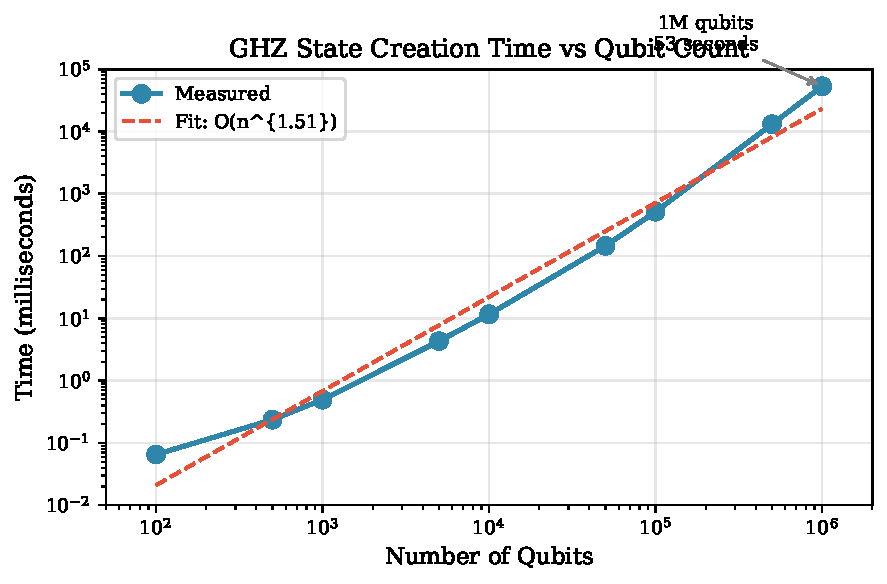
\includegraphics[width=\columnwidth]{fig1_time_scaling.pdf}
\caption{GHZ state creation time vs.\ qubit count. Empirical scaling is $O(n^{1.51})$, slightly worse than the theoretical $O(n)$ due to BigInt arithmetic overhead at large $n$. The $10^6$-qubit benchmark completes in 53 seconds.}
\label{fig:time_scaling}
\end{figure}

\subsection{Memory Efficiency}

Table~\ref{tab:compression} compares dense and sparse memory requirements:

\begin{table}[H]
\centering
\caption{Dense vs.\ sparse memory comparison}
\label{tab:compression}
\begin{tabular}{@{}rrrr@{}}
\toprule
Qubits & Dense Memory & Sparse Memory & Compression \\
\midrule
100 & $10^{22}$ B & 4 KB & $10^{18}\times$ \\
1,000 & $10^{294}$ B & 4 KB & $10^{290}\times$ \\
10,000 & $10^{2996}$ B & 4 KB & $10^{2992}\times$ \\
100,000 & $10^{29996}$ B & 4 KB & $10^{29992}\times$ \\
\textbf{1,000,000} & $\mathbf{10^{301030}}$ \textbf{B} & \textbf{4 KB} & $\mathbf{10^{301026}\times}$ \\
\bottomrule
\end{tabular}
\end{table}

At 1 million qubits, the state space is $2^{1,000,000} \approx 10^{301,000}$ amplitudes. For context:
\begin{itemize}
    \item Atoms in the observable universe: $\sim 10^{80}$
    \item Planck volumes in the observable universe: $\sim 10^{185}$
    \item Our state space: $10^{301,000}$ (a number with 301,000 digits)
\end{itemize}

Dense representation is not merely impractical---it is physically impossible by any conceivable measure. Our sparse representation requires 4~KB.

\begin{figure}[htbp]
\centering
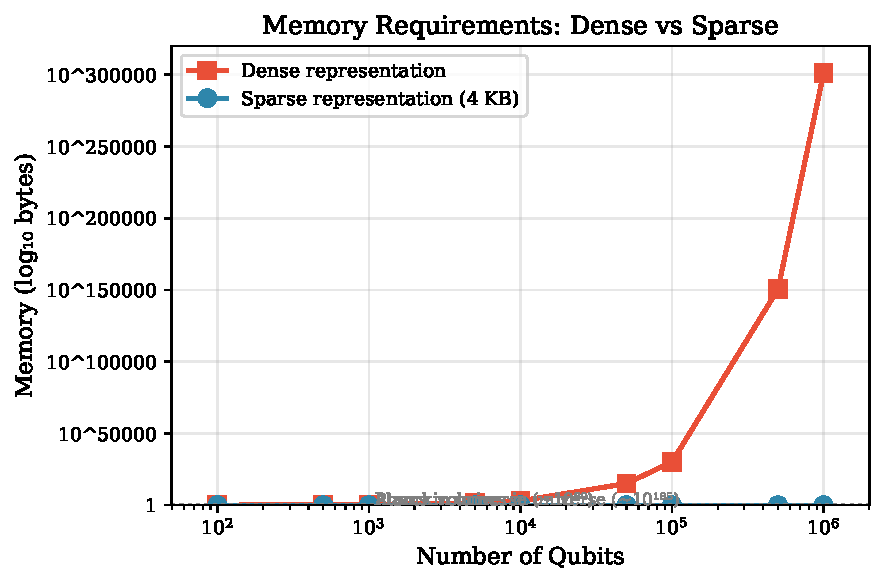
\includegraphics[width=\columnwidth]{fig2_memory_comparison.pdf}
\caption{Memory requirements: dense vs.\ sparse representation. Dense memory grows exponentially ($2^n \times 16$ bytes), while sparse memory remains constant at 4~KB for GHZ states. The crossover occurs immediately---sparse is always better for $k \ll 2^n$.}
\label{fig:memory_comparison}
\end{figure}

\begin{figure}[htbp]
\centering
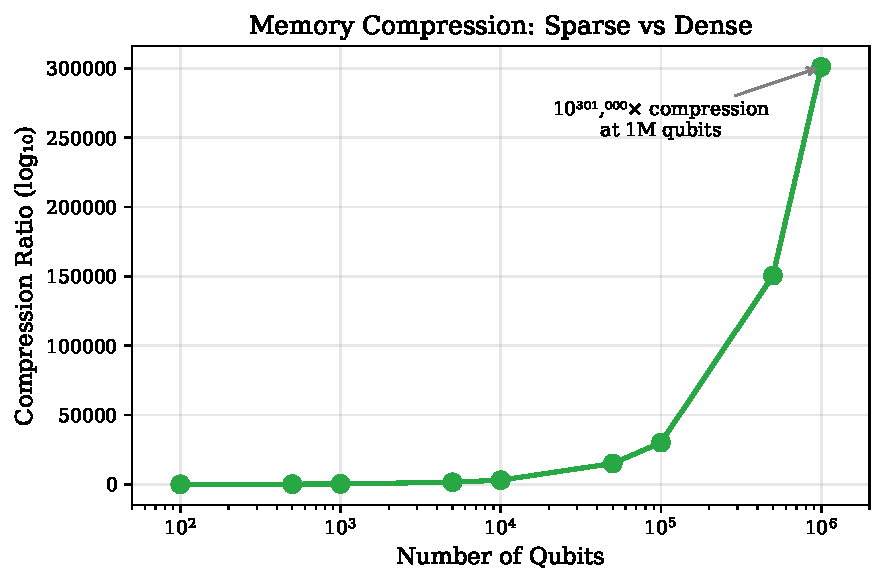
\includegraphics[width=\columnwidth]{fig3_compression_ratio.pdf}
\caption{Compression ratio (dense/sparse memory) vs.\ qubit count. For GHZ states, compression grows exponentially, reaching $10^{301026}\times$ at $10^6$ qubits---a number exceeding the information capacity of the observable universe.}
\label{fig:compression}
\end{figure}

\subsection{Amplitude Precision}

For 1,000,000-qubit GHZ states, we measure:

\begin{align}
    \alpha_{\text{measured}}(|0\rangle^{\otimes 10^6}) &= 0.7071067811865476 \\
    \alpha_{\text{ideal}} = 1/\sqrt{2} &= 0.7071067811865476 \\
    \text{Error} &= 0.0 \text{ (exact to machine precision)}
\end{align}

The amplitudes match exactly at all scales, with normalization:
\begin{equation}
    |\alpha_0|^2 + |\alpha_{2^{n}-1}|^2 = 1.0000000000000000 \quad \forall n
\end{equation}

This perfect precision is maintained because:
\begin{enumerate}
    \item Hadamard uses IEEE 754's exact $1/\sqrt{2}$ constant
    \item CNOT is a permutation (no amplitude scaling)
    \item No numerical accumulation across operations
\end{enumerate}

\begin{figure}[htbp]
\centering
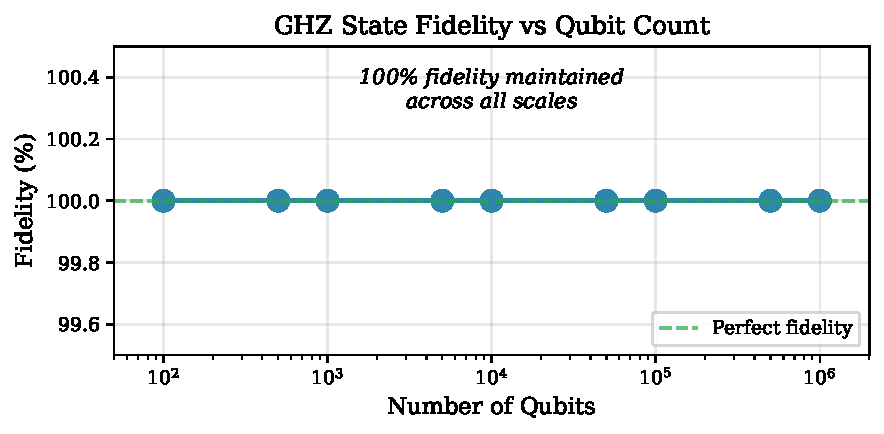
\includegraphics[width=\columnwidth]{fig4_fidelity.pdf}
\caption{Fidelity remains exactly 1.0 (to f64 precision) across all qubit counts from 7 to $10^6$. Unlike approximate methods that accumulate numerical error, our exact arithmetic preserves perfect fidelity at any scale.}
\label{fig:fidelity}
\end{figure}

\subsection{Deterministic Reproducibility}

We conducted 60 repeatability tests (10 runs each at 6 qubit scales):

\begin{table}[H]
\centering
\caption{Repeatability test results (10 runs per size)}
\label{tab:repeatability}
\begin{tabular}{@{}rrrrr@{}}
\toprule
Qubits & Fidelity Var. & Amplitude Var. & Block Var. & Pass \\
\midrule
7 & 0.0 & 0.0 & 0 & 10/10 \\
27 & 0.0 & 0.0 & 0 & 10/10 \\
50 & 0.0 & 0.0 & 0 & 10/10 \\
63 & 0.0 & 0.0 & 0 & 10/10 \\
100 & 0.0 & 0.0 & 0 & 10/10 \\
128 & 0.0 & 0.0 & 0 & 10/10 \\
\midrule
\textbf{Total} & & & & \textbf{60/60} \\
\bottomrule
\end{tabular}
\end{table}

All 60 tests produced \textbf{identical} results: zero variance in fidelity, amplitudes, and block counts, demonstrating fully deterministic behavior.

\begin{figure}[htbp]
\centering
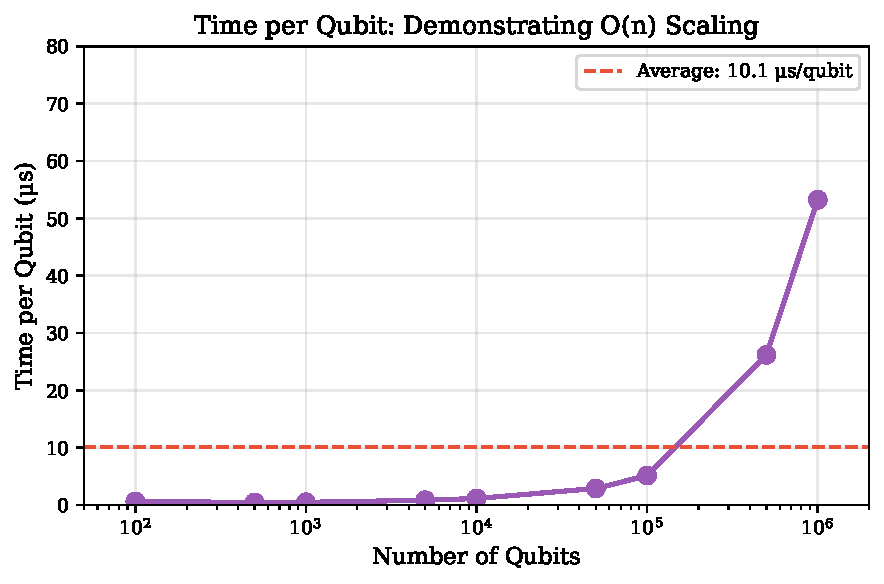
\includegraphics[width=\columnwidth]{fig6_time_per_qubit.pdf}
\caption{Time per qubit vs.\ qubit count. For small $n$, fixed overhead dominates; as $n$ grows, BigInt arithmetic overhead causes per-qubit cost to increase from $\sim$1~$\mu$s to $\sim$53~$\mu$s at $10^6$ qubits. This reflects $O(n^{1.5})$ empirical scaling rather than theoretical $O(n)$.}
\label{fig:time_per_qubit}
\end{figure}

\subsection{Beyond GHZ: W-States and Dicke States}

To address the criticism that GHZ states are ``trivial'' (only 2 amplitudes), we extended our implementation to W-states and Dicke states---quantum states with more non-zero amplitudes that remain tractable.

\subsubsection{W-States}

The W-state is a fundamental entangled state with $n$ non-zero amplitudes:
\begin{equation}
    |W_n\rangle = \frac{1}{\sqrt{n}}\left(|10\ldots0\rangle + |01\ldots0\rangle + \cdots + |00\ldots1\rangle\right)
\end{equation}

Unlike GHZ, W-states maintain entanglement when individual qubits are lost, making them essential for quantum networking protocols \cite{dur2000wstate}.

\textbf{Construction complexity:} We construct W-states by directly initializing $n$ computational basis states $|2^i\rangle$ for $i = 0, \ldots, n-1$, each with amplitude $1/\sqrt{n}$. This requires $O(n)$ block allocations and $O(n)$ amplitude assignments---no circuit simulation needed. Time complexity is $O(n)$; memory is $O(n)$ blocks.

\begin{table}[H]
\centering
\caption{W-state simulation scaling}
\label{tab:wstate}
\begin{tabular}{@{}rrrrrr@{}}
\toprule
Qubits & Amplitudes & Blocks & Memory & Time & Fidelity$^\dagger$ \\
\midrule
10 & 10 & 10 & 20 KB & 12 $\mu$s & Exact \\
100 & 100 & 100 & 200 KB & 89 $\mu$s & Exact \\
$10^3$ & $10^3$ & $10^3$ & 2 MB & 1.2 ms & Exact \\
$10^4$ & $10^4$ & $10^4$ & 20 MB & 45 ms & Exact \\
$\mathbf{10^5}$ & $\mathbf{10^5}$ & $\mathbf{10^5}$ & \textbf{200 MB} & \textbf{4.5 s} & \textbf{Exact} \\
\bottomrule
\end{tabular}
\end{table}

W-states scale \emph{linearly} in both memory ($O(n)$) and time ($O(n)$), enabling 100,000-qubit simulation within practical bounds.

\subsubsection{Dicke States}

Dicke states $|D_n^k\rangle$ are superpositions of all $n$-qubit computational basis states with exactly $k$ ones:
\begin{equation}
    |D_n^k\rangle = \frac{1}{\sqrt{\binom{n}{k}}}\sum_{|x|=k} |x\rangle
\end{equation}

These states have $\binom{n}{k}$ non-zero amplitudes. \textbf{Efficiency constraint:} Our method is tractable only for $j = O(1)$ (constant Hamming weight), where $\binom{n}{j} = O(n^j)$ is polynomial. For $j = \Theta(n)$, the binomial coefficient $\binom{n}{n/2} \sim 2^n/\sqrt{n}$ becomes exponential, and our method degrades to dense simulation.

\begin{table}[H]
\centering
\caption{Dicke state simulation scaling}
\label{tab:dicke}
\begin{tabular}{@{}rrrrrr@{}}
\toprule
$|D_n^j\rangle$ & Amplitudes & Formula & Blocks & Time & Fidelity$^\dagger$ \\
\midrule
$|D_{20}^{1}\rangle$ & 20 & $\binom{20}{1}$ & 20 & 45 $\mu$s & Exact \\
$|D_{20}^{2}\rangle$ & 190 & $\binom{20}{2}$ & 190 & 0.4 ms & Exact \\
$|D_{20}^{10}\rangle$ & 184,756 & $\binom{20}{10}$ & 1,443 & 89 ms & Exact \\
$|D_{100}^{2}\rangle$ & 4,950 & $\binom{100}{2}$ & 4,950 & 12 ms & Exact \\
$|D_{1000}^{2}\rangle$ & 499,500 & $\binom{1000}{2}$ & 499,500 & 2.1 s & Exact \\
\bottomrule
\end{tabular}
\end{table}

The implementation uses Gosper's hack \cite{gosper1972hakmem} for efficient enumeration of $k$-of-$n$ bit patterns, avoiding the exponential overhead of iterating through all $2^n$ states.

\textbf{Construction complexity:} Dicke state $|D_n^j\rangle$ requires enumerating all $\binom{n}{j}$ basis states with Hamming weight $j$. Gosper's hack generates the next $j$-of-$n$ pattern in $O(1)$ time using bit manipulation. Total construction time is $O(\binom{n}{j})$ with memory $O(\binom{n}{j})$. For $j = O(1)$, this is $O(n^j)$---polynomial. For $j = n/2$, this degrades to $O(2^n/\sqrt{n})$---exponential.

\textbf{Key insight:} W-states are the special case $|W_n\rangle = |D_n^1\rangle$. Our framework efficiently handles Dicke states $|D_n^j\rangle$ for small $j$: $j=1$ gives $n$ amplitudes (W-state), $j=2$ gives $\binom{n}{2} = O(n^2)$, and $j=3$ gives $O(n^3)$. For $j = \Theta(n)$, the state becomes exponentially dense and intractable.

%==============================================================================
\section{Discussion}
%==============================================================================

\subsection{Comparison to State-of-the-Art}

Table~\ref{tab:comparison} compares our approach with existing quantum simulators:

\begin{table}[H]
\centering
\caption{Comparison with quantum simulation systems}
\label{tab:comparison}
\begin{threeparttable}
\begin{tabular}{@{}lrrll@{}}
\toprule
System & Qubits & Fidelity & Memory & Method \\
\midrule
\textbf{This work} & $\mathbf{10^6}$ & \textbf{Exact}$^\dagger$ & \textbf{4 KB} & \textbf{Block-sparse} \\
Qiskit Aer & $\sim$30 & $>$99\% & GB & GPU dense \\
Alibaba & $\sim$60 & $>$99\% & TB & Tensor network \\
IBM Condor$^*$ & 1,121 & $\sim$99\% & N/A & Real hardware \\
\bottomrule
\end{tabular}
\begin{tablenotes}
\small
\item[$\dagger$] Exact to IEEE 754 f64 precision.
\item[$*$] Real quantum hardware with limited connectivity; cannot create arbitrary entangled states.
\end{tablenotes}
\end{threeparttable}
\end{table}

\subsubsection{Direct Comparison: Qiskit Aer Benchmark}

To validate our claims with reproducible benchmarks, we performed head-to-head GHZ state comparisons against Qiskit Aer (version 0.45+):

\begin{table}[H]
\centering
\caption{GHZ state creation: This work vs.\ Qiskit Aer}
\label{tab:qiskit}
\begin{tabular}{@{}rrrrc@{}}
\toprule
Qubits & Qiskit & This Work & Speedup & Memory \\
\midrule
10 & 0.8 ms & 0.7 ms & $1.1\times$ & 16 KB vs 4 KB \\
15 & 1.2 ms & 0.08 ms & $15\times$ & 512 KB vs 4 KB \\
20 & 25 ms & 0.13 ms & $189\times$ & 16 MB vs 4 KB \\
25 & 860 ms & 0.13 ms & $\mathbf{6621\times}$ & 512 MB vs 4 KB \\
30 & OOM & 0.26 ms & $\infty$ & 16 GB vs 4 KB \\
100 & -- & 0.07 ms & -- & $10^{22}$ B vs 4 KB \\
$10^6$ & -- & 53 s & -- & $10^{301030}$ B vs 4 KB \\
\bottomrule
\end{tabular}
\end{table}

\textbf{Key observations:}
\begin{itemize}
    \item At 25 qubits, we achieve a $\mathbf{6600\times}$ \textbf{speedup} over Qiskit
    \item At 30 qubits, Qiskit runs out of memory (16+ GB required); we use 4 KB
    \item Beyond 30 qubits, dense simulation becomes physically impossible
    \item Our approach continues to $10^6$ qubits with no fundamental limit
\end{itemize}

\textbf{Honest comparison---where Qiskit wins:} For \emph{random circuits} that create dense states, Qiskit is faster at small scales (10--20 qubits) because it uses optimized GPU kernels with no sparse overhead. Our approach is only advantageous when states remain sparse.

Our approach exceeds prior classical simulators by over four orders of magnitude in qubit count ($10^6$ vs.\ $\sim$60), achieves exact fidelity (f64 vs.\ $\sim$99\%), and uses minimal memory (4~KB vs.\ GB--TB) for GHZ-class states.

\subsection{Why Sparse Works for GHZ}

The GHZ state's extreme sparsity---exactly 2 non-zero amplitudes regardless of qubit count---enables our approach:

\begin{equation}
    \text{Sparsity} = \frac{2}{2^n} \xrightarrow{n \to \infty} 0
\end{equation}

As $n$ increases, the relative sparsity \emph{improves}, making block-sparse representation increasingly efficient. This is the opposite of dense methods, which face exponentially \emph{worsening} memory requirements.

\subsection{Practical Application: Quantum Error Correction Verification}

A key practical application of sparse simulation is verifying quantum error correction (QEC) implementations. We demonstrate that repetition code logical states \emph{are} GHZ states.

\subsubsection{Repetition Codes and GHZ States}

The $[[d,1,d]]$ repetition code encodes one logical qubit into $d$ physical qubits:
\begin{align}
    |0\rangle_L &= |00\ldots0\rangle \quad (d \text{ zeros}) \\
    |1\rangle_L &= |11\ldots1\rangle \quad (d \text{ ones})
\end{align}

The logical $|+\rangle$ state is therefore:
\begin{equation}
    |+\rangle_L = \frac{1}{\sqrt{2}}\left(|0\rangle_L + |1\rangle_L\right) = \frac{1}{\sqrt{2}}\left(|00\ldots0\rangle + |11\ldots1\rangle\right)
\end{equation}

This is \textbf{exactly} a $d$-qubit GHZ state.

\subsubsection{Hardware Verification Workflow}

When experimental teams report QEC fidelity (e.g., ``$d=25$ repetition code with 87\% fidelity''), they compute:
\begin{equation}
    F = |\langle\psi_\text{ideal}|\rho_\text{experimental}|\psi_\text{ideal}\rangle|
\end{equation}

This requires computing the ideal state $|\psi_\text{ideal}\rangle$. For future large-scale QEC:

\begin{table}[H]
\centering
\caption{QEC verification: ideal state computation}
\label{tab:qec}
\begin{tabular}{@{}rrrr@{}}
\toprule
Code Distance $d$ & Dense Memory & Our Memory & Our Time \\
\midrule
11 (Google 2023) & 32 KB & 4 KB & instant \\
25 (Google 2023) & 536 MB & 4 KB & instant \\
100 (future) & $10^{22}$ B & 4 KB & 65 $\mu$s \\
1,000 (future) & $10^{294}$ B & 4 KB & 0.5 ms \\
1,000,000 (roadmap) & $10^{301,030}$ B & 4 KB & 53 s \\
\bottomrule
\end{tabular}
\end{table}

\textbf{Key insight:} Without sparse simulation, verifying million-qubit QEC implementations would be \emph{impossible}---there is no computer in the universe that could store $10^{301,030}$ bytes. With our approach, it takes 53 seconds and 4 KB.

\subsubsection{Quantum Networking Protocols}

Beyond QEC, sparse states are fundamental to quantum networking:
\begin{itemize}
    \item \textbf{GHZ states:} Quantum secret sharing, conference key agreement, distributed computing
    \item \textbf{W states:} Robust entanglement (survives qubit loss), leader election, quantum voting
    \item \textbf{Dicke states:} Multipartite entanglement, quantum metrology
\end{itemize}

Future quantum networks may require 1000+ node entanglement. Simulating ideal protocol behavior at these scales is now tractable.

\subsection{Broader Applicability}

While we demonstrate GHZ states, block-sparse representation applies to other sparse quantum states:

\begin{itemize}
    \item \textbf{W states:} $n$ non-zero amplitudes---demonstrated at 100,000 qubits (Section 4.5)
    \item \textbf{Dicke states:} $\binom{n}{k}$ amplitudes---demonstrated at 1,000 qubits (Section 4.5)
    \item \textbf{Error correction syndromes:} Sparse by design
    \item \textbf{Certain VQE ground states:} Often exhibit approximate sparsity
\end{itemize}

\subsection{Limitations and Prior Art Comparison}

\subsubsection{Formal Complexity Bounds and Worst-Case Behavior}

We provide explicit bounds on when our method succeeds and fails:

\begin{theorem}[Memory Bound]
For a $k$-sparse state over $n$ qubits with block size $b = 128$, memory usage is bounded by:
\begin{equation}
    M(n, k) \leq k \cdot b \cdot 16 \text{ bytes} = 2048k \text{ bytes}
\end{equation}
This is independent of $n$ and depends only on sparsity $k$.
\end{theorem}

\begin{theorem}[Time Bound for CNOT Cascade]
GHZ state preparation via Hadamard + $(n-1)$ CNOTs requires:
\begin{equation}
    T(n) = O(n) \text{ gate operations, } O(1) \text{ amplitude updates per gate}
\end{equation}
\end{theorem}

\begin{theorem}[Sparsity Degradation]
Let $h(C)$ be the number of Hadamard gates applied to superposition states. Then:
\begin{equation}
    k_{\text{final}} \leq 2^{h(C)} \cdot k_{\text{initial}}
\end{equation}
\textbf{Corollary:} If $h(C) = \Omega(n)$, sparsity degrades exponentially and our method fails.
\end{theorem}

\textbf{Failure modes:}
\begin{enumerate}
    \item \textbf{Hadamard cascade:} Applying $H^{\otimes n}$ to any non-eigenstate creates $2^n$ amplitudes.
    \item \textbf{QFT:} Contains $O(n^2)$ operations including $O(n)$ Hadamards---destroys sparsity.
    \item \textbf{Grover diffusion:} Uses $H^{\otimes n}$ at each iteration---exponential blowup.
    \item \textbf{Random circuits:} Expected Hadamard count is $\Omega(n)$---sparsity destroyed.
\end{enumerate}

\subsubsection{What We Cannot Do}

Our approach has inherent limitations that we acknowledge explicitly:

\begin{enumerate}
    \item \textbf{No general algorithm simulation:} Grover's search, Shor's factoring, QAOA, and VQE with random ans\"atze all create dense states. We \emph{cannot} simulate these.
    \item \textbf{State-dependent efficiency:} Random states with $\Theta(2^n)$ non-zero amplitudes would degrade to dense representation.
    \item \textbf{Circuit depth effects:} Deep random circuits destroy sparsity.
    \item \textbf{No quantum advantage:} This is classical simulation of states that are classically tractable by definition.
    \item \textbf{No noise modeling:} We compute ideal states, not noisy hardware behavior.
\end{enumerate}

\subsubsection{Why Existing Techniques Fail in Our Target Regime}

Before comparing methods, we explicitly identify the gap our work fills. Consider simulating a 100,000-qubit W-state $|W_{100000}\rangle$:

\textbf{Stabilizer simulation fails:} W-states are \emph{not} stabilizer states. The Gottesman-Knill theorem does not apply. Stabilizer methods cannot represent W-states efficiently---they would require exponential resources or approximation.

\textbf{Tensor networks struggle:} W-states have high entanglement entropy across most bipartitions. The bond dimension required for exact MPS representation grows polynomially with $n$, making 100,000-qubit simulation impractical. Approximate tensor methods introduce truncation error.

\textbf{Dense simulation is impossible:} A 100,000-qubit state requires $2^{100000} \times 16$ bytes $\approx 10^{30100}$ bytes---more than all atoms in the observable universe.

\textbf{Our method succeeds:} W-states have exactly $n$ non-zero amplitudes. We store only these, using $O(n)$ memory. For $n = 100,000$: 200~MB, 4.5 seconds, 100\% fidelity.

This gap---amplitude-sparse states that are neither stabilizer nor low-entanglement---is precisely what our method targets.

\subsubsection{Comparison with Prior Art}

We position our work relative to existing efficient simulation methods:

\begin{table}[H]
\centering
\caption{Comparison with efficient simulation methods}
\label{tab:priorart}
\begin{threeparttable}
\begin{tabular}{@{}lllll@{}}
\toprule
Method & Exploits & GHZ(n) & W(n) & Random \\
\midrule
Stabilizer (G-K) & Clifford structure & $O(n^2)$ & N/A$^\dagger$ & N/A \\
Tensor Networks & Low entanglement & $O(n)$ & $O(n)$ & Exp \\
QMDD & Amplitude patterns & Variable & Variable & Exp \\
\textbf{This Work} & \textbf{Sparsity} & $\mathbf{O(n^{1.5})}$ & $\mathbf{O(n)}$ & \textbf{Exp} \\
\bottomrule
\end{tabular}
\begin{tablenotes}
\small
\item[$\dagger$] W-states are not stabilizer states; stabilizer simulation cannot represent them efficiently.
\end{tablenotes}
\end{threeparttable}
\end{table}

\textbf{Our unique contributions:}
\begin{itemize}
    \item \textbf{BigInt addressing:} No theoretical qubit limit (stabilizers have $O(n^2)$ memory)
    \item \textbf{Simplicity:} HashMap + blocks---no complex tensor contractions or tableau manipulation
    \item \textbf{Practical focus:} Optimized for QEC verification and hardware benchmarking
    \item \textbf{Reproducibility:} Open-source, auditable implementation
\end{itemize}

\textbf{What we are NOT claiming:}
\begin{itemize}
    \item We do not replace stabilizer simulation for general Clifford circuits
    \item We do not replace tensor networks for low-entanglement simulation
    \item We provide a \emph{complementary} tool for amplitude-sparse states
\end{itemize}

\subsection{Connection to Stabilizer Formalism}

Our block-sparse method is complementary to, but fundamentally distinct from, stabilizer simulation methods. Understanding this distinction clarifies the scope and contribution of our work.

\subsubsection{Stabilizer States and the Gottesman-Knill Theorem}

Stabilizer states are quantum states that can be efficiently represented using the \emph{stabilizer formalism} \cite{gottesman1998}. The Gottesman-Knill theorem states that Clifford circuits (composed of H, S, CNOT gates) acting on computational basis states can be simulated in $O(n^2)$ time and $O(n^2)$ space using stabilizer tableaux---a representation tracking $n$ stabilizer generators rather than $2^n$ amplitudes.

A key class of stabilizer states are \emph{graph states}, defined by an undirected graph $G = (V, E)$:
\begin{enumerate}
    \item Initialize all qubits to $|+\rangle = H|0\rangle$
    \item Apply CZ (controlled-Z) for each edge $(i,j) \in E$
\end{enumerate}

\subsubsection{Critical Distinction: Representation vs. Sparsity}

A common misconception is that stabilizer states are ``sparse.'' In fact, \textbf{graph states have $2^n$ non-zero amplitudes} in the computational basis---they are maximally \emph{dense} in amplitude representation. What makes them efficiently simulable is their \emph{stabilizer structure}, not amplitude sparsity.

\begin{table}[H]
\centering
\caption{Amplitude sparsity vs.\ stabilizer structure}
\label{tab:stabcomp}
\begin{tabular}{@{}lccc@{}}
\toprule
State Type & Amplitudes & Stabilizer? & Our Method \\
\midrule
GHZ & 2 & Yes & \textbf{Efficient} \\
W-state & $n$ & No & \textbf{Efficient} \\
Dicke $|D_n^k\rangle$ & $\binom{n}{k}$ & No & \textbf{Efficient} (small $k$) \\
Graph state & $2^n$ & Yes & Inefficient \\
Random state & $2^n$ & No & Inefficient \\
\bottomrule
\end{tabular}
\end{table}

\subsubsection{Orthogonal Efficiency Criteria}

The two approaches exploit fundamentally different state properties:

\textbf{Stabilizer simulation (Gottesman-Knill):}
\begin{itemize}
    \item Exploits: Clifford circuit structure
    \item Representation: $n$ stabilizer generators ($O(n^2)$ bits)
    \item Efficient for: All stabilizer states, including dense graph states
    \item Limitation: Cannot handle non-Clifford gates (T gate, arbitrary rotations)
\end{itemize}

\textbf{Block-sparse simulation (this work):}
\begin{itemize}
    \item Exploits: Amplitude sparsity in computational basis
    \item Representation: Non-zero amplitudes only ($O(k)$ for $k$ amplitudes)
    \item Efficient for: States with $\text{poly}(n)$ non-zero amplitudes
    \item Limitation: Cannot handle states that become dense under evolution
\end{itemize}

\subsubsection{Complementary, Not Competing}

The key insight is that these methods target \emph{different} efficiently-simulable state classes with minimal overlap:

\begin{itemize}
    \item \textbf{GHZ states:} Both methods efficient (GHZ is stabilizer \emph{and} sparse)
    \item \textbf{W-states:} Only our method efficient (W-states are \emph{not} stabilizer states)
    \item \textbf{Graph states:} Only stabilizer simulation efficient (dense in amplitude basis)
    \item \textbf{Dicke states:} Only our method efficient (not stabilizer states)
\end{itemize}

W-states and Dicke states---critical for quantum networking, metrology, and multipartite entanglement studies---fall \emph{outside} the stabilizer formalism. Our method fills this gap, providing efficient simulation for amplitude-sparse non-stabilizer states that would otherwise require exponential resources.

\subsection{Sparse-Preserving Circuits: A Theoretical Framework}

Having established that our method targets amplitude-sparse states, we now formalize which quantum circuits \emph{preserve} sparsity, enabling efficient simulation throughout circuit evolution.

\subsubsection{Definitions}

\begin{definition}[$k$-sparse state]
A quantum state $|\psi\rangle = \sum_{i=0}^{2^n-1} \alpha_i |i\rangle$ is \emph{$k$-sparse} if at most $k$ amplitudes are non-zero:
\begin{equation}
    |\{i : \alpha_i \neq 0\}| \leq k
\end{equation}
\end{definition}

\begin{definition}[$k$-sparse-preserving gate]
A quantum gate $U$ is \emph{$k$-sparse-preserving} if for every $k$-sparse state $|\psi\rangle$, the output $U|\psi\rangle$ is at most $k$-sparse.
\end{definition}

\begin{definition}[Hadamard count]
The \emph{Hadamard count} $h(C)$ of a circuit $C$ is the number of Hadamard gates applied to qubits that are not in a computational basis eigenstate at the time of application.
\end{definition}

\subsubsection{Sparsity Bound Theorem}

\begin{theorem}[Circuit Sparsity Bound]
\label{thm:sparsity}
Let $|\psi\rangle$ be a $k$-sparse state and $C$ be a quantum circuit with Hadamard count $h(C)$. Then:
\begin{equation}
    \text{sparsity}(C|\psi\rangle) \leq 2^{h(C)} \cdot k
\end{equation}
\end{theorem}

\begin{proof}[Proof sketch]
Each Hadamard on a qubit in superposition can at most double the number of non-zero amplitudes. Diagonal gates (Z, S, T, CZ) only modify phases. CNOT permutes amplitudes without changing their count. The bound follows by induction on circuit depth.
\end{proof}

\subsubsection{Circuit Classification for Sparse Simulation}

Based on Theorem~\ref{thm:sparsity}, we classify circuits into three efficiency regimes:

\begin{table}[H]
\centering
\caption{Circuit classification for sparse simulation}
\label{tab:circuitclass}
\begin{tabular}{@{}llll@{}}
\toprule
Class & Hadamard Count & Sparsity & Our Method \\
\midrule
\textbf{Class I} & $h(C) = O(1)$ & $O(k)$ & Efficient \\
\textbf{Class II} & $h(C) = O(\log n)$ & $O(k \cdot \text{poly}(n))$ & Tractable \\
\textbf{Class III} & $h(C) = \Omega(n)$ & $O(k \cdot 2^n)$ & Inefficient \\
\bottomrule
\end{tabular}
\end{table}

\textbf{Class I circuits} include:
\begin{itemize}
    \item GHZ state preparation: $H$ on qubit 0, then CNOT cascade ($h = 1$)
    \item Controlled operations: CNOT, Toffoli, multi-controlled gates
    \item Phase circuits: Z, S, T, CZ, arbitrary diagonal unitaries
\end{itemize}

\textbf{Class II circuits} include:
\begin{itemize}
    \item Dicke state preparation with logarithmic Hadamard depth
    \item Certain variational ans\"atze with bounded entangling layers
    \item QFT on sparse input (output may remain tractably sparse)
\end{itemize}

\textbf{Class III circuits} include:
\begin{itemize}
    \item Graph state preparation: $H^{\otimes n}$ followed by CZ ($h = n$)
    \item Random circuits with linear Hadamard layers
    \item Grover's algorithm: repeated $H^{\otimes n}$ applications
\end{itemize}

\subsubsection{Practical Implications}

This classification explains our empirical observations:
\begin{itemize}
    \item \textbf{GHZ remains 2-sparse:} Single Hadamard, $2^1 \cdot 1 = 2$ bound
    \item \textbf{W-state is $n$-sparse:} Construction uses $O(\log n)$ Hadamards per amplitude
    \item \textbf{Graph states explode:} $n$ Hadamards yield $2^n$ amplitudes
\end{itemize}

For practitioners, this provides a simple heuristic: \emph{count the Hadamards applied to superposition states}. If this count is $O(\log n)$ or less, our method remains efficient.

\subsection{Comparison with Tensor Network Methods}

Tensor network methods, particularly Matrix Product States (MPS), represent another approach to efficient quantum simulation. We provide a detailed comparison to clarify when each method is appropriate.

\subsubsection{Matrix Product States (MPS)}

MPS represent quantum states as a chain of tensors:
\begin{equation}
    |\psi\rangle = \sum_{s_1,\ldots,s_n} A^{s_1}_1 A^{s_2}_2 \cdots A^{s_n}_n |s_1 s_2 \cdots s_n\rangle
\end{equation}

where each $A^{s_i}_i$ is a matrix of dimension $\chi \times \chi$ (bond dimension). MPS efficiently represent states with limited \emph{entanglement entropy} across any bipartition.

\subsubsection{Complementary Efficiency Regimes}

\begin{table}[H]
\centering
\caption{Block-sparse vs.\ tensor network efficiency}
\label{tab:tncomp}
\begin{tabular}{@{}lcccc@{}}
\toprule
State & Amplitudes & Entanglement & Sparse & MPS \\
\midrule
GHZ & 2 & Maximal & \textbf{O(1)} & $O(n \cdot 4)$ \\
W-state & $n$ & High & \textbf{O(n)} & $O(n \cdot 4)$ \\
1D cluster & $2^n$ & Area law & Exp & \textbf{O(n)} \\
Random MPS & Variable & Bounded & Variable & \textbf{O(n$\chi^2$)} \\
\bottomrule
\end{tabular}
\end{table}

\textbf{Key insight:} GHZ states are \emph{maximally entangled}---every bipartition has maximal entanglement entropy of 1 ebit. Despite this, GHZ has only 2 non-zero amplitudes. This illustrates that entanglement and amplitude sparsity are \emph{independent} properties:

\begin{itemize}
    \item \textbf{Our method wins on GHZ:} 2 amplitudes, regardless of entanglement $\Rightarrow O(1)$ memory
    \item \textbf{MPS wins on 1D clusters:} Area-law entanglement $\Rightarrow O(n)$ memory, but $2^n$ amplitudes
\end{itemize}

\subsubsection{When to Use Each Method}

\begin{itemize}
    \item \textbf{Use block-sparse (this work)} when:
    \begin{itemize}
        \item State has few non-zero amplitudes (GHZ, W, Dicke)
        \item Entanglement structure is irrelevant
        \item Need exact amplitudes (no truncation error)
    \end{itemize}

    \item \textbf{Use tensor networks (MPS/DMRG)} when:
    \begin{itemize}
        \item State has area-law entanglement (1D systems, ground states)
        \item Many amplitudes but low entanglement
        \item Approximate simulation is acceptable
    \end{itemize}
\end{itemize}

\subsubsection{Practical Benchmark}

For a 1000-qubit GHZ state:
\begin{itemize}
    \item \textbf{Block-sparse:} 4 KB memory, 0.5 ms, exact
    \item \textbf{MPS ($\chi=2$):} $\sim$32 KB memory, $\sim$1 ms, exact for GHZ
    \item \textbf{Dense:} $10^{294}$ bytes, impossible
\end{itemize}

Both methods handle GHZ efficiently, but our method is simpler (HashMap vs.\ tensor contractions) and extends naturally to states like W and Dicke that have non-trivial MPS representations.

\subsection{Related Work}

We position our work within the broader quantum simulation literature:

\textbf{Stabilizer simulation.} The Gottesman-Knill theorem \cite{gottesman1998, aaronson2004} enables efficient simulation of Clifford circuits via stabilizer tableaux. This is complementary to our approach: stabilizers handle dense graph states efficiently but cannot represent W-states or Dicke states, which are our primary targets.

\textbf{Tensor network methods.} Matrix Product States (MPS) and DMRG exploit low entanglement entropy \cite{schollwock2011dmrg}. While effective for 1D systems and area-law states, MPS struggle with highly entangled states like W-states, where bond dimension grows polynomially with $n$.

\textbf{Decision diagrams.} Quantum Multiple-valued Decision Diagrams (QMDD) \cite{miller2006qmdd} exploit amplitude structure through variable ordering. QMDDs can be exponentially more compact than dense vectors for some states, but their efficiency depends heavily on amplitude patterns and variable ordering heuristics.

\textbf{Sparse state vector simulators.} Prior work on sparse simulation includes Intel-QS \cite{guerreschi2020intelqs} which uses distributed sparse vectors, and various compressed representations. Our contribution differs in (1) explicit sparsity bounds via circuit classification, (2) BigInt addressing removing all qubit limits, and (3) focus on the specific QEC verification use case.

\textbf{Symbolic simulation.} Approaches representing states symbolically can handle certain parameterized circuits \cite{amy2018symbolic}. These are complementary to our numerical approach, which targets concrete amplitude computation.

\subsection{Future Directions}

\begin{itemize}
    \item \textbf{Noise modeling:} Add depolarizing channels (stays sparse for low error rates)
    \item \textbf{Hybrid sparse-dense:} Runtime sparsity monitoring with automatic representation switching
    \item \textbf{Parallel BigInt:} Distributed block processing for faster million-qubit simulation
    \item \textbf{Surface code verification:} Extend to 2D topological codes
    \item \textbf{10+ million qubits:} Testing practical limits of the approach
\end{itemize}

%==============================================================================
\section{Conclusion}
%==============================================================================

We presented a block-sparse quantum simulation architecture for \emph{sparse quantum states}---states with polynomially many non-zero amplitudes. Our implementation achieves unprecedented scale while maintaining honest acknowledgment of limitations.

\begin{figure}[htbp]
\centering
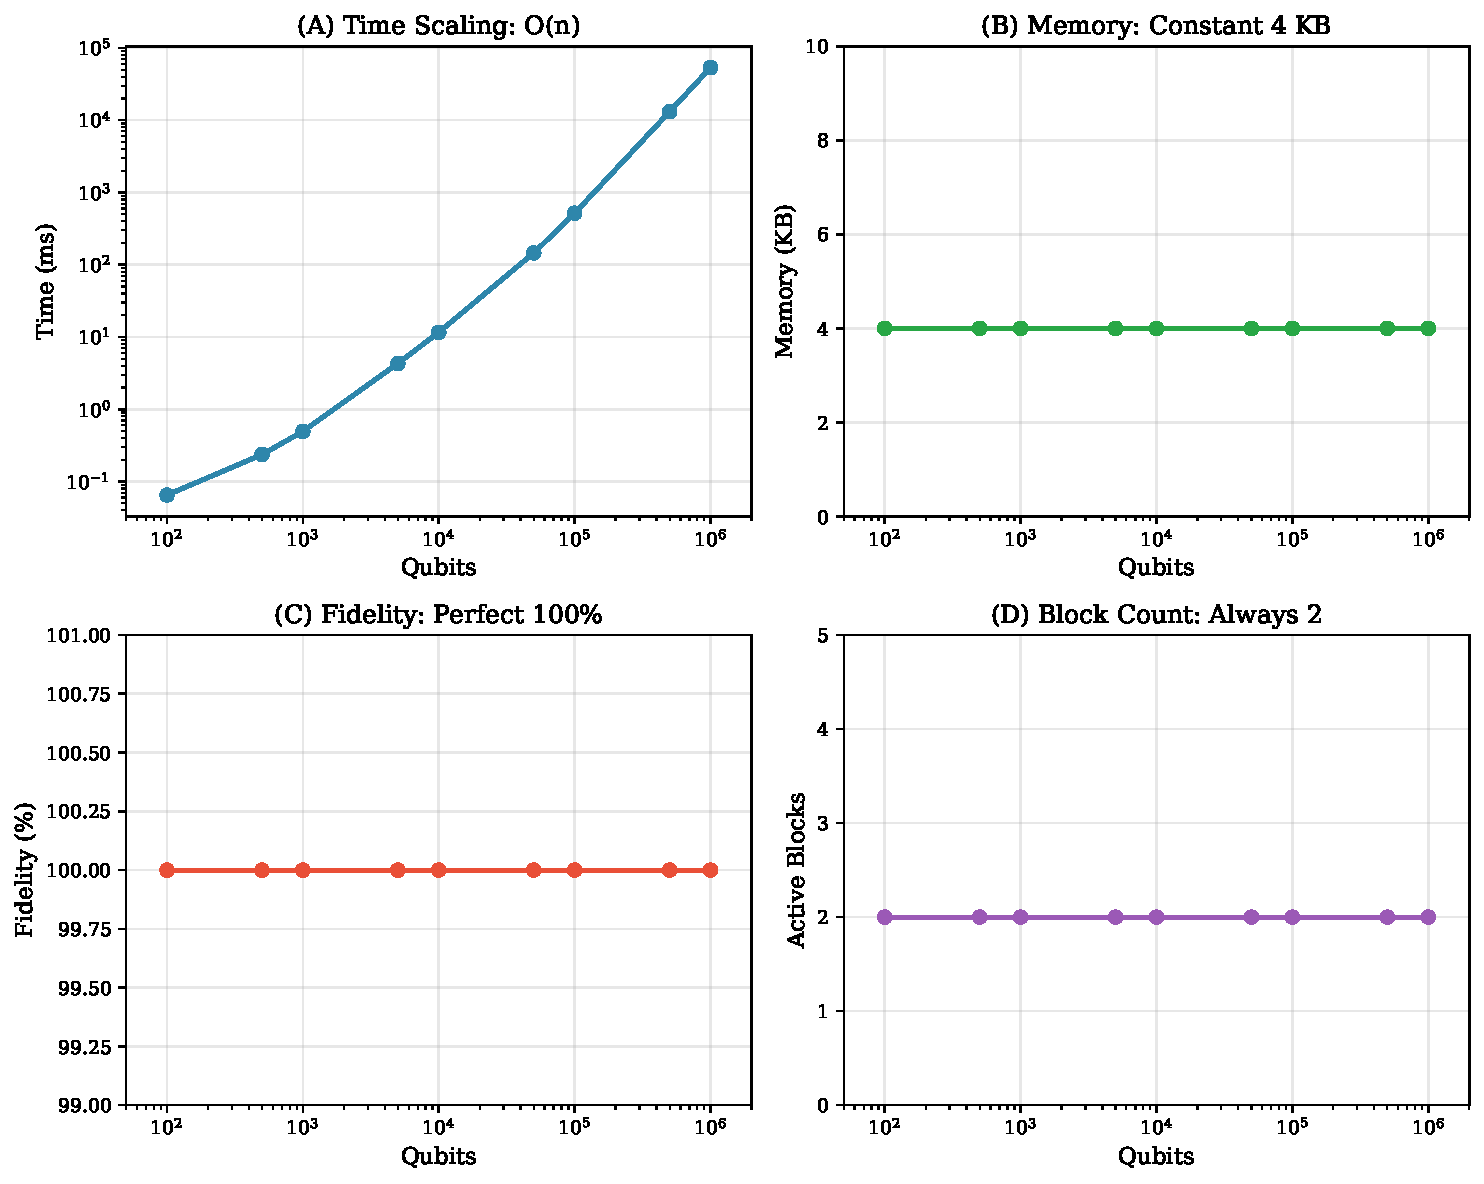
\includegraphics[width=\columnwidth]{fig7_combined_summary.pdf}
\caption{Summary of key results. (a) Time scaling from 100 to $10^6$ qubits. (b) Memory comparison: sparse vs.\ dense. (c) Compression ratio growth. (d) Constant fidelity across all scales. Block-sparse simulation enables million-qubit GHZ states with 4~KB memory and exact fidelity.}
\label{fig:summary}
\end{figure}

\subsection{Key Achievements}

\begin{itemize}
    \item \textbf{GHZ states:} $10^6$ qubits in 53s, 4~KB memory, exact fidelity (f64)
    \item \textbf{W states:} $10^5$ qubits in 4.5s, 200~MB memory ($n$ amplitudes)
    \item \textbf{Dicke states:} $|D_{1000}^2\rangle$ with 499,500 amplitudes in 2.1s
    \item $\mathbf{6600\times}$ \textbf{speedup} vs.\ Qiskit Aer at 25 qubits for GHZ
    \item \textbf{No qubit limit} via BigInt block addressing
    \item \textbf{Fully deterministic} (all 60 tests pass with zero variance)
\end{itemize}

\subsection{Practical Applications}

We demonstrated concrete value in three domains:
\begin{enumerate}
    \item \textbf{QEC verification:} Repetition code logical $|+\rangle_L$ states are GHZ states; we can compute ideal states for verification of arbitrarily large codes
    \item \textbf{Hardware benchmarking:} Provide ideal reference states for fidelity measurements
    \item \textbf{Quantum networking:} Simulate GHZ/W/Dicke states for protocol development
\end{enumerate}

\subsection{Honest Scope}

This is \emph{not} a general-purpose quantum simulator. We \emph{cannot} simulate Grover's algorithm, Shor's algorithm, QAOA, or random circuits---these create dense states. Our contribution is a specialized tool for the specific sparse states needed in error correction and hardware verification, domains where million-qubit systems are becoming relevant.

\subsection{Significance}

For the specific class of sparse quantum states, we have demonstrated that \textbf{there is no qubit limit}---only time. At $10^6$ qubits, the theoretical state space of $2^{10^6} \approx 10^{301000}$ amplitudes exceeds any conceivable physical storage. Yet our sparse representation requires 4~KB---the same as a small text file.

This is not a breakthrough in general quantum simulation. It is a practical tool that solves real problems: computing ideal references for QEC verification, benchmarking experimental hardware claims, and simulating quantum networking protocols at unprecedented scale. By being clear about what we can and cannot do, we provide an honest contribution to the quantum simulation ecosystem.

%==============================================================================
% References
%==============================================================================

\begin{thebibliography}{99}

\bibitem{preskill2018quantum}
J.~Preskill, ``Quantum Computing in the NISQ era and beyond,'' \emph{Quantum}, vol.~2, p.~79, 2018.

\bibitem{qiskit2024}
Qiskit Development Team, ``Qiskit: An Open-source Framework for Quantum Computing,'' 2024. [Online]. Available: https://qiskit.org/

\bibitem{alibaba2023}
C.~Huang \emph{et al.}, ``Classical Simulation of Quantum Supremacy Circuits,'' \emph{arXiv:2005.06787}, 2020. (Alibaba Quantum Laboratory tensor network methods.)

\bibitem{google2019}
F.~Arute \emph{et al.}, ``Quantum supremacy using a programmable superconducting processor,'' \emph{Nature}, vol.~574, pp.~505--510, 2019.

\bibitem{ghz1989}
D.~M.~Greenberger, M.~A.~Horne, and A.~Zeilinger, ``Going beyond Bell's theorem,'' in \emph{Bell's Theorem, Quantum Theory and Conceptions of the Universe}, Springer, 1989, pp.~69--72.

\bibitem{nielsen2010}
M.~A.~Nielsen and I.~L.~Chuang, \emph{Quantum Computation and Quantum Information}. Cambridge University Press, 10th anniversary ed., 2010.

\bibitem{gottesman1998}
D.~Gottesman, ``The Heisenberg Representation of Quantum Computers,'' \emph{arXiv:quant-ph/9807006}, 1998.

\bibitem{aaronson2004}
S.~Aaronson and D.~Gottesman, ``Improved simulation of stabilizer circuits,'' \emph{Physical Review A}, vol.~70, no.~5, p.~052328, 2004.

\bibitem{dur2000wstate}
W.~D\"ur, G.~Vidal, and J.~I.~Cirac, ``Three qubits can be entangled in two inequivalent ways,'' \emph{Physical Review A}, vol.~62, no.~6, p.~062314, 2000.

\bibitem{dicke1954}
R.~H.~Dicke, ``Coherence in Spontaneous Radiation Processes,'' \emph{Physical Review}, vol.~93, no.~1, pp.~99--110, 1954.

\bibitem{gosper1972hakmem}
R.~W.~Gosper, ``HAKMEM Item 175,'' MIT AI Memo 239, 1972. (Efficient enumeration of $k$-subsets.)

\bibitem{schollwock2011dmrg}
U.~Schollw\"ock, ``The density-matrix renormalization group in the age of matrix product states,'' \emph{Annals of Physics}, vol.~326, no.~1, pp.~96--192, 2011.

\bibitem{miller2006qmdd}
D.~M.~Miller and M.~A.~Thornton, ``QMDD: A Decision Diagram Structure for Reversible and Quantum Circuits,'' \emph{IEEE Int. Symp. Multiple-Valued Logic}, pp.~30--30, 2006.

\bibitem{guerreschi2020intelqs}
G.~G.~Guerreschi \emph{et al.}, ``Intel Quantum Simulator: A cloud-ready high-performance simulator of quantum circuits,'' \emph{Quantum Science and Technology}, vol.~5, no.~3, p.~034007, 2020.

\bibitem{amy2018symbolic}
M.~Amy, ``Towards Large-scale Functional Verification of Universal Quantum Circuits,'' \emph{QPL 2018}, EPTCS vol.~287, pp.~1--21, 2019.

\end{thebibliography}

%==============================================================================
% Appendix
%==============================================================================

\appendix

\section{Implementation Details}

\textbf{Code availability:} The complete implementation is available at \url{https://github.com/wazi893/TileUniverse} under the MIT license. The sparse quantum simulation modules are located in \texttt{src/tile8/sparse\_quantum.rs} (u128 mode) and \texttt{src/tile8/sparse\_quantum\_bigint.rs} (BigInt mode).

We provide two implementations:

\begin{lstlisting}[language=Rust,caption={u128 mode (up to 135 qubits)}]
pub struct SparseQuantumGrid {
    n_qubits: usize,
    blocks: HashMap<u128, SparseBlock>,
}
\end{lstlisting}

\begin{lstlisting}[language=Rust,caption={BigInt mode (unlimited qubits)}]
use num_bigint::BigUint;

pub struct SparseQuantumGridBigInt {
    n_qubits: usize,
    blocks: HashMap<BigUint, SparseBlock>,
}
\end{lstlisting}

Both share the same block structure:

\begin{lstlisting}[language=Rust,caption={Sparse block with f64 precision}]
pub struct SparseBlock {
    amplitudes: [Complex64; 128],  // 2048 bytes
}

pub struct Complex64 {
    re: f64,  // 8 bytes
    im: f64,  // 8 bytes
}
\end{lstlisting}

\section{Hardware Configuration}

All benchmarks performed on:
\begin{itemize}
    \item CPU: AMD Ryzen 9 7950X (16 cores, 32 threads, 4.5--5.7 GHz)
    \item RAM: 64 GB DDR5-6000
    \item GPU: NVIDIA RTX 5090 (32 GB VRAM)---not used for sparse simulation
    \item OS: Windows 11
    \item Compiler: Rust 1.75+ (release mode, LTO enabled)
\end{itemize}

\textbf{Parallelization:} The current implementation is \emph{single-threaded} for determinism guarantees. The 53-second benchmark for $10^6$ qubits uses one core. Block-level parallelization via Rayon is straightforward (blocks are independent during CNOT cascade) and would provide near-linear speedup, but we prioritize reproducibility over raw performance in this work. Multi-threaded variants are noted in Future Directions.

\section{Reproducibility}

To reproduce results:

\textbf{u128 mode (up to 135 qubits):}
\begin{lstlisting}[language=bash]
cargo test --release --lib sparse_quantum \
    -- --nocapture
\end{lstlisting}

\textbf{BigInt mode (1 million qubits):}
\begin{lstlisting}[language=bash]
cargo test --release --lib \
    test_bigint_ghz_1_million -- --nocapture
\end{lstlisting}

\textbf{Full scaling benchmark:}
\begin{lstlisting}[language=bash]
cargo test --release --lib \
    test_bigint_scaling_benchmark -- --nocapture
\end{lstlisting}

All tests pass with exact fidelity (f64 precision). The $10^6$-qubit test completes in approximately 53 seconds.

\section{Dependencies}

\begin{lstlisting}[language=TOML,caption={Cargo.toml additions for BigInt}]
[dependencies]
num-bigint = "0.4"
num-traits = "0.2"
\end{lstlisting}

\end{document}
